\documentclass[a4paper]{article}

\usepackage[english]{babel}
\usepackage[utf8]{inputenc}
\usepackage{amsmath}
\usepackage{graphicx}
\usepackage[colorinlistoftodos]{todonotes}
\usepackage{listings}
\usepackage{hyperref}

\title{Statistical Inference Course Project, part 1: Simulation}

\author{Daniel Kudlowiez Franch}

\begin{document}
\maketitle

This part of the project focuses in simulating sequences following an exponential distribution with the $\lambda$ parameter set to 0.2. Both the mean and standard deviation of this distribution are given by $1/\lambda$. Each simulation will sample the distribution 40 times and then the sample mean and standard deviation will be compared with the expected theoretical values.

The following code will make a thousand simulations of the process of sampling 40 times:

\begin{small}
\begin{lstlisting}[frame = single]
set.seed(4)
lambda <- 0.2
numSimulations <- 1000
sampSize <- 40
simulation <- matrix(rexp(numSimulations*sampSize,rate=lambda),
				numSimulations,	sampSize)
simMeans <- rowMeans(simulation)
\end{lstlisting}
\end{small}

The resulting distribution is shown in the following figure.

\begin{figure}[h!]
\centering
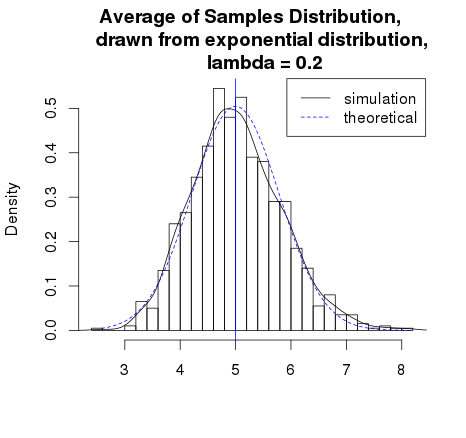
\includegraphics[width = 0.5\textwidth]{hist_part_1.png}
\end{figure}

This distribution is centered at 4.982616, while theoretically it should be at $\lambda^{-1} = $ 5. The variance obtained from the distribution is 0.657568 while the theoretical value would be $\sigma^2/n = 1/(\lambda^2n) = 1/(0.2^240) = 0.625$.

The distribution of means follows a normal distribution, as it would be expected by the Central Limit Theorem. The figure above displays the histogram of the obtained distribution and the theoretical normal distribution that would be expected. Furthermore, the Q-Q Plot below also suggests the normality of the distribution.

\begin{figure}[h!]
\centering
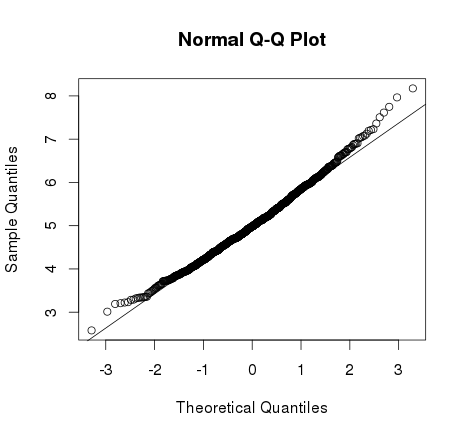
\includegraphics[width = 0.5\textwidth]{qqplot_part_1.png}
\end{figure}

Lastly, the confidence interval for this measurement of the mean is evaluated for $1/\lambda = \bar{X} \pm 1.96\frac{S}{\sqrt{n}}$.

\begin{figure}[h!]
\centering
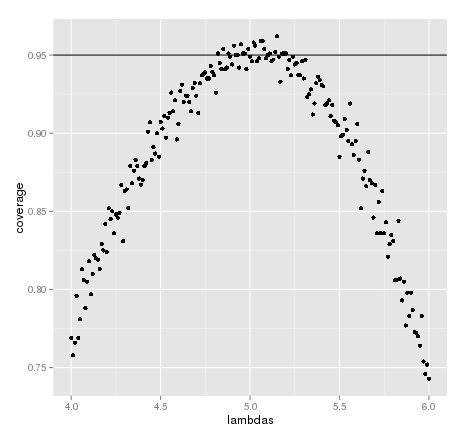
\includegraphics[width = 0.5\textwidth]{confidence_part_1.png}
\end{figure}

From this figure it is possible to see that the 95\% confidence interval for the rate parameter fall in the interval close to the value 5 at least 95\% of the time.

This report, figures and the code used to do the simulation and generate the plots can be found at $https://github.com/franchenstein/statistical_inference/$.

\end{document}
